\section{Applicability of the vertically global shearing box}\label{global_corr}
In \S\ref{analytical} we used the vertically global shearing box
\citep[VGSB,][]{mcnally14} to make analytical progress. % Here, we discuss limitations of this approach.   
The main difference between the linear problem in the VGSB 
and the radially-local approximation
(Eq. \ref{lin_mass}---\ref{lin_energy}) adopted in our numerical study
is the absence of  terms associated with the radial disk structure in
the former framework. These terms appear in the energy, mass and radial momentum
equations and are reproduced here for convenience,
% Using the notation and disk models in the main text, the
% energy, density and $r$ momentum equations become 
\begin{align}
  \ii \sigma W  &=c _s^2(r_0, z)\left( \left.\frac{\p\ln\rho}{\p
      z}\right|_0 \delta v_z + \frac{\gamma}{\Gamma} \frac{d\delta
    v_z}{dz}\right) + \left[\ii k_xc_s^2(r_0,z)
  \frac{\gamma}{\Gamma} + \hat{g}_c\left.\frac{1}{\rho}\frac{\p P}{\p
      r}\right|_0\right]\delta v_x  +
\frac{1}{t_c}\left(W-\frac{Q}{\Gamma}\right),\label{gcorr_terms1}\\
\ii \sigma Q &= c_s^2(r_0,z)\left(\ii k_r + \hat{g}_c
  \left.\frac{\p\ln{\rho}}{\p r}\right|_0\right)\delta v_x + c _s^2(r_0, z)\left( \left.\frac{\p\ln\rho}{\p
      z}\right|_0 \delta v_z + \frac{d\delta
    v_z}{dz}\right),\label{gcorr_terms2} \\
\ii \sigma \delta v_x & = \ii k_x W  -
\hat{g}_c\frac{1}{c_s^2(r_0,z)}\left.\frac{1}{\rho}\frac{\p P}{\p
  r}\right|_0Q - 2\Omega(r_0,z)\delta v_y,\label{gcorr_terms3}
\end{align}
where subscript $0$ denotes evaluation at $r=r_0$.

In the VGSB, the terms proportional to $\hat{g}_c$ are ignored. For a
power-law disk, these radial gradients are $O(r^{-1})$, and they
appear in comparison with terms of $O(k_x)$. The neglected terms 
therefore have a relative magnitude of $O(\epsilon/\khat)$. This is
small for thin disks ($\epsilon\ll1$) and/or small radial wavelengths
($\khat\gg 1$). 

%  To obtain the
% linear problem in the VGSB, we take the radially-local 
% approximation further and formally set $\hat{g}_c=0$, $r\to x$ and
% $k_r\to k_x$. It is clear that this approximation improves with
% increasing $|k_x|$.   

\subsection{Spurious growth of adiabatic perturbations in the VGSB}\label{analytic_adia} 
An important caveat of the VGSB is that it cannot be used in the
adiabatic limit. We explain this by setting  $\beta\to\infty$ in
Eq. \ref{vertiso_gov_nondim}, which can then be written as 
% For adiabatic perturbations ($\gamma>1$, $\beta\to\infty$) we may
% simply use the Soilberg-Hoiland critera to assess stability
% (\S\ref{solberg}). Nevertheless, we briefly consider this case in the
% local framework to demonstrate its limitations. For $\beta\to\infty$
% the parameter $\chi = 1/\gamma$ and Eq. \ref{vertiso_gov_nondim} can
% be written as   
\begin{align}
  0 =\dd v_z^{\prime\prime} + \left(1 + \ii \epsilon q
    \hat{k}\right)\left(\ln\rho^{\prime}\delta v_z\right)^\prime
  +\left\{\hat{\sigma}^2\left(\frac{1}{\gamma}+\hat{k}^2\right) 
    -\left(\frac{\gamma-1}{\gamma}\right)\left[\ln\rho^{\prime\prime}+\hat{k}^2\left(1-\frac{\ii\epsilon  
          q}{\hat{k}}\right)\ln\rho^{\prime 2}\right]\right\}\delta v_z.\label{adia_iso3}
\end{align}
We multiply Eq. \ref{adia_iso3} by $\rho\delta v_z^*$ and
integrate vertically, assume boundary terms vanish when integrating by
parts, to obtain
\begin{align}
  \hat{\sigma}^2\left(\frac{1}{\gamma} +
    \hat{k}^2\right)\int_{\zhat_1}^{\zhat_2}\rho|\delta
  v_z|^2 d\zhat 
  =&  \left(\frac{\gamma-1}{\gamma}\right)
  \int_{\zhat_1}^{\zhat_2}\rho|\delta v_z^\prime|^2 d\zhat
  +\frac{1}{\gamma}\int_{\zhat_1}^{\zhat_2}\frac{1}{\rho}|(\rho\delta
  v_z)^\prime|^2 d\zhat\notag\\
&+
  \left(\frac{\gamma-1}{\gamma}\right)\hat{k}^2\left(1-\frac{\ii\epsilon
      q}{\hat{k}}\right) \int_{\zhat_1}^{\zhat_2}\rho\ln\rho^{\prime
    2}|\delta v_z|^2 d\zhat
+ \ii\epsilon q \hat{k}
  \int_{\zhat_1}^{\zhat_2}\ln\rho^\prime(\rho\delta v_z^*)^\prime
  \delta v_z d\zhat.\label{adia_integral}
\end{align}
When $q\equiv0$, all the terms on the right-hand-side (RHS) are real. Then
$\hat{\sigma}^2$ is real, and  $\hat{\sigma}^2>0$ if $\gamma>1$. As
expected, a sub-adiabatically stratified disk is stable in the absense
of vertical shear. 

However, in the presence of vertical shear $q\neq0$,
Eq. \ref{adia_integral} suggests $\hat{\sigma}$ is complex for real
$\khat$, which implies the possibility of instability, regardless of
how much $\gamma$ deviates from unity. This is contradicts the second 
Solberg-Hoiland criterion (Eq. \ref{solberg2}), which states that
instability in the adiabatic limit requires the disk to be close to
neutrally stratified. %also need real freq^2 in adia limit 
This is because the VGSB retains the destabilizing effect of vertical shear
($\p_z\Omega$) from the global disk, but ignores the global radial disk
structure responsible for it. Nevertheless, we demonstrate below that
this inconsistency is unimportant for the vertical shear instability,
which occurs for $\beta\ll1$. 

% To 
% avoid this, we must restrict our attention to short thermal relaxation
% timescales ($\beta\lesssim1$) and/or neutrally-stratified disks
% ($\gamma=\Gamma$) when $q\neq0$. 

\subsection{Effect of global radial gradients}
% We may also reverse the above procedure by reinstating the `global
% correction' terms proportional to $\hat{g}_c$ in the linear VGSB
% equations. Of course, doing so implies the basic state is not uniform
% in $x$, which would be inconsistent with the full VGSB equations in
% equilibrium. Nevertheless, we illustrate in Fig. \ref{gcorr_compare} the effect of
% these global radial gradients on the growth rate of the fundamental
% VSI.  

% The global correction terms do not change the qualitative dependence
% of the fundamental VSI growth rates on the thermal relaxation
% timescale. The difference is negligble for $\beta\lesssim 1$ (i.e.
% fast thermal relaxation). The critical relaxation timescale for the
% fundamental VSI is unaffected by these global radial radients. 

% However, in the adiabatic limit $\beta\to\infty$ the linear VGSB
% equations give a positive growth rate as discussed in
% \S\ref{analytic_adia}, which is inconsistent with the second
% Solberg-Hoiland criterion (Eq. \ref{solberg2}). The correct behaviour
% ($\nu\to0$ as $\beta\to\infty$) is obtained with global correction.  

In  Fig. \ref{gcorr_compare}, we demonstrate the effect of the global radial gradient terms
proportional to $\hat{g}_c$ in 
Eq. \ref{gcorr_terms1}---\ref{gcorr_terms3} by calculating the
fundamental VSI growth rates using three approaches. We compute growth rates from the dispersion
relation Eq. \ref{relax_disp}, which utilizes the VGSB;  from the
full linear problem (Eq. \ref{lin_mass}---\ref{lin_energy}) with
$\hat{g}_c=0$ (i.e. the linear VGSB equations); and from the full
linear problem with $\hat{g}_c=1$.  

All three methods give similar behavior, and growth rates are in close
agreement for $\beta\lesssim 1$. Differences arise for
$\beta\gtrsim1$, and as $\beta\to\infty$ the VGSB framework gives a
(spurious) positive growth rate as expected from the discussion
above. Inclusion of the global radial gradient terms results in the
correct behavior  ($\nu\to0$ as $\beta\to\infty$).  

\begin{figure}
  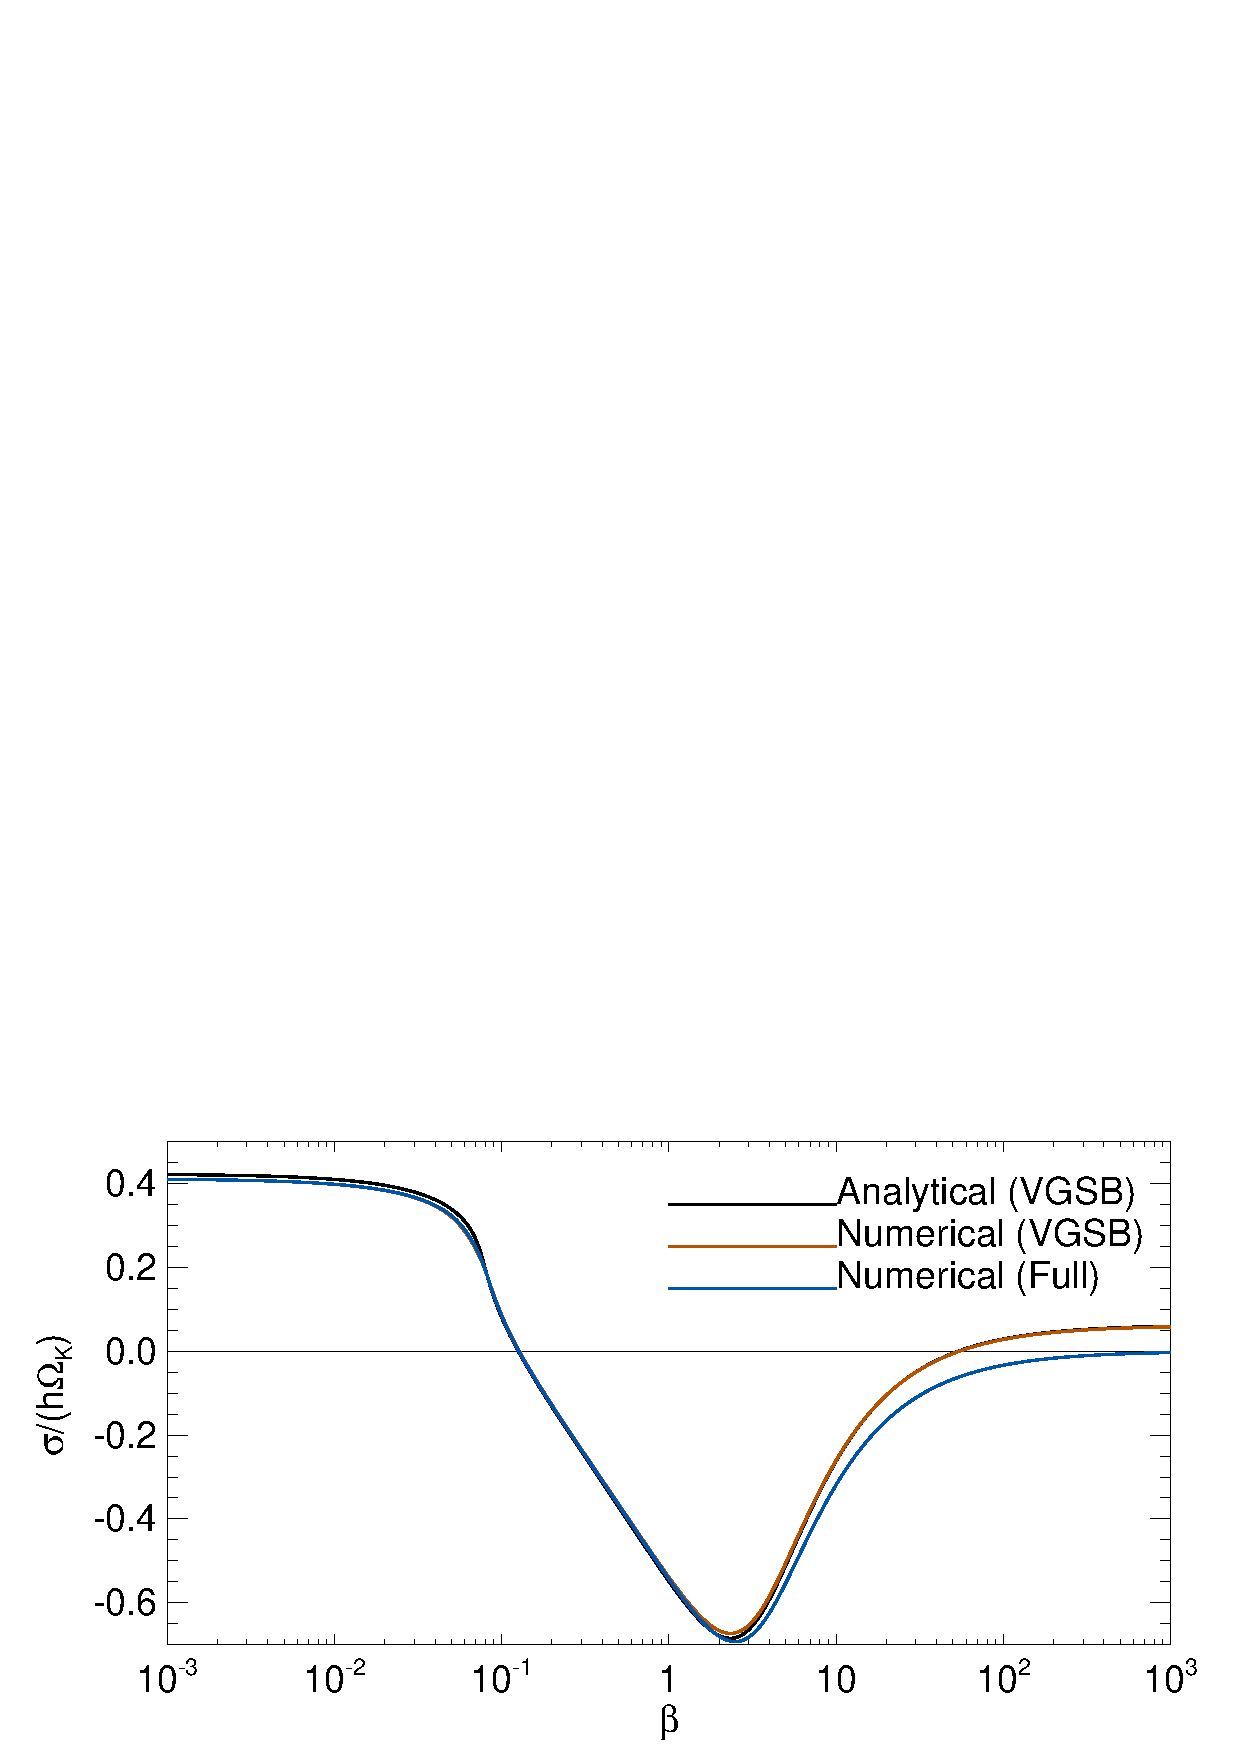
\includegraphics[width=\linewidth,clip=true,trim=0cm 0.0cm 0cm
  0cm]{figures/gcorr_compare} 
  \caption{Growth rate of the fundamental VSI mode as a function of
    the thermal relaxation time $\beta$. The `Analytical (VGSB)' curve
    is calculated from the dispersion relation Eq. \ref{relax_disp};
    the `Numerical (VGSB)' curve is obtained by numerically solving
    Eq. \ref{lin_mass}---\ref{lin_energy} with $\hat{g}_c=0$
    (which defines the linear VGSB equations); and the `Numerical
    (Full)' curve is obtained by numerically solving
    Eq. \ref{lin_mass}---\ref{lin_energy}  with $\hat{g}_c=1$, which
    accounts for the radial disk structure.  
% computed from the linear VGSB equations used in
%     the main text (dotted) and that including additional global
%     radial gradient terms in
%     Eq. \ref{gcorr_terms1}---\ref{gcorr_terms3} (solid). 
    The disk parameters are $\Gamma=1.011$,
    $\gamma=1.4$ and $(p,q,\epsilon)=(-1.5,-1,0.05)$. The perturbation
    wavenumber is $\khat=30$. 
    \label{gcorr_compare}}  
\end{figure}

Fig. \ref{gcorr_compare} shows that provided we consider $\beta\ll1$,
then the VGSB framework is an adequate approximation. It is
interesting to note that there is a thermal relaxation timescale that
maximizes the mode decay rate. Here, it is $\beta\simeq2$ or about
$0.3$ orbital periods. This is, in fact, consistent with Fig. 12 of
\cite{nelson13}.  




%nevertheless we have calculated
%plot growth rate v.s. bcool 



\section{Full governing equation for vertically isothermal disks in
  the VGSB}\label{adia_improve}
% \section{Improving the nearly-Keplerian approximation for adiabatic
%   disks}\label{adia_improve}
In \S\ref{approx_gov} we made the replacement $D\to\Omega_k^2$ before
eliminating variables to obtain a single equation for $\delta v_z$,
Eq. \ref{vertiso_gov}.  This procedure ignores the vertical dependence of
$D=\kappa^2(z) - \sigma^2$. We show here that this has no significant
consequence for thin disks. 

In the global disk with $\Gamma=1$ we have
\begin{align}\label{dkappa2}
  \frac{\p\kappa^2}{\p z} = 4 \frac{\p\Omega^2}{\p z} + r\frac{\p}{\p
    r}\frac{\p\Omega^2}{\p z} = -
  \frac{\p\ln\rho}{\p z}\frac{qc_s^2}{r^2} \left(2 + q +
    \frac{z^2/r^2-2}{z^2/r^2+1}\right). 
\end{align}
For the local problem we may then write
\begin{align}
  \frac{dD}{dz}  = - \frac{d\ln\rho}{dz}\frac{qc_s^2}{r^2}F(z;q),
\end{align}
where the function $F$ corresponds to the bracket in
Eq. \ref{dkappa2}. This function varies from $F=q$ at $z=0$ to $F\to
3+q$ as $|z|\to\infty$, i.e. its magnitude is of order unity. 

 Eliminating $W$ and $Q$ from Eq. \ref{ode_w}---\ref{ode_Q} and
 Eq. \ref{lin_vz} for vertically isothermal disks, retaining the
 vertical dependence of $D$ and including thermal relaxation, we
 obtain 
\begin{align}
  0 =& \frac{d^2\delta v_z}{dz^2} + \left[1 + \frac{\ii k_x c_s^2
      q}{Dr} - \frac{k_x^2c_s^2}{\left(k_x^2c_s^2 + \chi
        D\right)}\frac{qc_s^2F}{Dr^2}\right]\frac{d\ln\rho}{dz}\frac{d\delta
    v_z}{dz} \notag\\
  &+ \left\{\sigma^2\left(\frac{k_x^2}{D} +
      \frac{\chi}{c_s^2}\right) + \left(\chi + \frac{\ii k_x c_s^2
        q}{Dr}\right)\frac{d^2\ln\rho}{dz^2} -
    \frac{c_s^2}{D}\left(\frac{d\ln\rho}{dz}\right)^2\left(k_x^2 -
      \frac{\ii k_x q}{r}\right)
   \left[\left(1-\chi\right) +
     \frac{\chi}{\left(k_x^2c_s^2 + \chi D\right)}\frac{qc_s^2 F}{r^2}\right] 
   \right\}\delta v_z,
\end{align}
where we recall $\chi = \left(1-\ii\sigma t_c\right)/\left(1-\ii\sigma
t_c \gamma\right)$. Making the low-frequency approximation with the
replacement $D\to \Omega_k^2$ gives, in terms of dimensionless
variables,
\begin{align}
   &\delta v_z ^{\prime\prime} + \left[1 + \ii\epsilon q\hat{k} -
    \frac{ \hat{k}^2}{
      \left(\hat{k}^2+\chi\right)}q \epsilon^2F\right]\ln\rho^{\prime}\delta v_z^\prime +
  \left\{\left(\chi + \ii \epsilon q
      \hat{k}\right)\ln\rho^{\prime\prime} - \ln\rho^{\prime
      2}\left(\khat^2 -
      \ii\epsilon
      q\hat{k}\right)\left[1 - \chi +
      \frac{\chi}{\left(\hat{k}^2+\chi\right)}q\epsilon^2F\right]\right\}\delta v_z \notag\\&=
  -\hat{\sigma}^2\left(\hat{k}^2+\chi\right)\delta v_z\label{adia_diso3}.
\end{align}   
Eq. \ref{adia_diso3} differs from Eq. \ref{vertiso_gov_nondim} by terms
proportional to $\epsilon^2$. For a thin disk, $\epsilon\ll1$, so
neglecting these terms has no qualitative effect on the discussion in 
\S\ref{analytic_relax}.  This issue does not
arise for isothermal perturbations discussed in \S\ref{iso_discuss}
since in that case we work with a governing equation for $W$ instead. 

% \section{Alternative inference of instability in the presence of weak
%   vertical shear}\label{pert_theory}
% We can also investigate the destabilizing effect of vertical shear
% without explicitly solving the full governing equation,
% Eq. \ref{iso_ode3}. We first
% consider a system with $q\equiv0$, for which the eigenfunctions are
% Hermite polynomials and the real eigenfrequencies are known. We then
% perturb this system by introducing a weak vertical shear ($|q|\ll1$)
% and linearize the governing equation. This procedure is
% \begin{align}   
%   q \to 0 + \delta q,\quad
%   W \to \He_n + \delta W,\quad
%   \hat{\sigma} \to \hat{\sigma} + \delta\hat{\sigma}. 
% \end{align}
% %where for this exercise we restore $\sigma$ as the eigenfrequency. 

% Linearizing the integral relation Eq. \ref{integral_relation1} in the
% thin-disk limit, and taking the
% imaginary part, we have
% \begin{align}
%   2\hat{\sigma}\imag(\delta\hat{\sigma})
%   \left(1+\hat{k}^2\right) \int_{-\infty}^{\infty} w(\zhat)
%   \He_n^2(\hat{z}) d\hat{z}
%   = \delta q \epsilon \hat{k} 
%   \int_{-\infty}^{\infty}
%   w(\zhat)\hat{z}\He_n(\hat{z})\He_n^\prime(\zhat) d\hat{z}
% \end{align}
% Recognizing $\hat{z} = \He_1(\hat{z})$ and using $\He_n^\prime = n
% \He_{n-1}$ we have
%  \begin{align}
%    2\hat{\sigma}\imag(\delta\hat{\sigma})
%    \left(1+\hat{k}^2\right) \int_{-\infty}^{\infty} w(\zhat)
%    \He_n^2(\hat{z}) d\hat{z}
%    =\delta q \epsilon \hat{k} 
%    \int_{-\infty}^{\infty}
%    w(\zhat)\He_1(\hat{z})\He_n(\hat{z})n\He_{n-1}(\hat{z})d\hat{z}. 
%  \end{align}

% Finally, we evaluate the integrals using the results
% \begin{align}
%   \int_{-\infty}^{\infty}
%   w(\xi) \He_k(\xi)\He_l(\xi) d\xi = \sqrt{2\pi}k!\delta_{kl} \quad
% % \end{align}
% \text{and} \quad
% % \begin{align}
%   \int_{-\infty}^{\infty}
%   w(\xi) \He_m(\xi)\He_k(\xi)\He_l(\xi) d\xi =
%   \frac{\sqrt{2\pi}m!k!l!}{(j-m)!(j-k)!(j-l)!}, 
% \end{align}
% where $j = (m+k+l)/2$. We then obtain
%  \begin{align}
%    2\hat{\sigma}\imag(\delta\hat{\sigma})
%   \left(1+\hat{k}^2\right) = \delta q \epsilon \hat{k} n.
%  \end{align}
% Inserting the original eigenfrequency $\hat{\sigma} = \pm
% \sqrt{n}(1+\hat{k}^2)^{-1/2}$ gives
% \begin{align}
%   \imag(\delta\hat{\sigma})= \pm \frac{1}{2}\delta q \epsilon
%   \sqrt{n} \frac{\hat{k}}{\sqrt{1+\hat{k}^2}}. 
% \end{align}
% This result agrees with Eq. \ref{simple_growth} in the limit
% $|q|\to0$. 
% %for $n=1$, since the
% %function $\He_1$ solves the governing equation exactly. 
% For $\hat{k}\gg 1$ we have
% \begin{align}
%   \imag(\delta\hat{\sigma})\simeq \pm \frac{1}{2}\delta q \epsilon
%   \sqrt{n} \sgn{\hat{k}}. 
% \end{align}




% Differentiating Eq. \ref{adia_iso1} properly gives
% \begin{align}
%   \left(D + \gamma k_x^2 c_s^2\right)\frac{d\Delta}{dz}=& D
%   \frac{d^2\delta v_z}{dz^2} + k_x^2c_s^2\left[\frac{\gamma}{\left(D + \gamma k_x^2 c_s^2\right)}\frac{dD}{dz} + \ii
%     \frac{d\ln\rho}{dz}\left(\ii +
%       \frac{q}{k_xr}\right)\right]\frac{d\delta v_z}{dz}\notag\\
%   &+ \ii k_x^2 c_s^2 \left(\ii +
%       \frac{q}{k_xr}\right)\left[\frac{d^2\ln\rho}{dz^2} -
%       \frac{1}{\left(D + \gamma
%           k_x^2c_s^2\right)}\frac{dD}{dz}\frac{d\ln\rho}{dz}\right]\delta
%     v_z. \label{adia_diso1}
% \end{align}
% The terms that were ignored in deriving Eq. \ref{adia_iso3} are those
% proportional to $dD/dz$ in Eq. \ref{adia_diso1}. Now, in the global
% disk with $\Gamma=1$ we have
% \begin{align}\label{dkappa2}
%   \frac{\p\kappa^2}{\p z} = 4 \frac{\p\Omega^2}{\p z} + r\frac{\p}{\p
%     r}\frac{\p\Omega^2}{\p z} = -
%   \frac{\p\ln\rho}{\p z}\frac{qc_s^2}{r^2} \left(2 + q +
%     \frac{z^2/r^2-2}{z^2/r^2+1}\right). 
% \end{align}
% For the local problem we may then write
% \begin{align}
%   \frac{dD}{dz}  = - \frac{d\ln\rho}{dz}\frac{qc_s^2}{r^2}F(z;q),
% \end{align}
% where the function $F$ corresponds to the bracket in
% Eq. \ref{dkappa2}. This function varies from $F=q$ at $z=0$ to $F\to
% 3+q$ as $|z|\to\infty$, i.e. its magnitude is of order unity. 
% % We estimate the
% % importance of these terms by noting that 
% % \begin{align}
% %   \frac{dD}{dz}\equiv \frac{d\kappa^2}{dz} \simeq \frac{d\Omega^2}{dz}
% %   = - \frac{d\ln\rho}{dz}\frac{qc_s^2}{r^2},
% % \end{align}
% % for thin disks. 
% Eq. \ref{adia_diso1} becomes
% \begin{align}
% \left(D + \gamma k_x^2 c_s^2\right)\frac{d\Delta}{dz}=& D
%   \frac{d^2\delta v_z}{dz^2} - k_x^2c_s^2\frac{d\ln\rho}{dz}\left[ 1 - 
%       \frac{\ii q}{k_xr}  +  \frac{\gamma q c_s^2F}{r^2\left(D +
%         \gamma k_x^2 c_s^2\right)}\right]\frac{d\delta
%     v_z}{dz}\notag\\ 
%   &- k_x^2 c_s^2 \left(1 - 
%       \frac{\ii q}{k_xr}\right)\left[\frac{d^2\ln\rho}{dz^2} + 
%       \frac{qc_s^2F}{r^2\left(D + \gamma
%           k_x^2c_s^2\right)}\left(\frac{d\ln\rho}{dz}\right)^2\right]\delta
%     v_z. \label{adia_diso2}
% \end{align}
% Since $D\sim \Omega_k^2$ in the low-frequency limit, we 
% see from Eq. \ref{adia_diso2} that the neglected terms are
% $O(\epsilon^2)$. We can make this explicit by combining
% Eq. \ref{adia_diso1}---\ref{adia_diso2} and Eq. \ref{adia_iso2}, then
% set $D\to\Omega_k^2$. In terms of non-dimensional variables, the result
% is  
% \begin{align}
%    &\delta v_z ^{\prime\prime} + \left(1 + \ii\epsilon q\hat{k} -
%     \frac{\gamma q \epsilon^2\hat{k}^2F}{1+\gamma
%       \hat{k}^2}\right)\ln\rho^{\prime}\delta v_z^\prime +
%   \left[\left(\frac{1}{\gamma} + \ii \epsilon q
%       \hat{k}\right)\ln\rho^{\prime\prime} - \hat{k}^2\left(1 -
%       \frac{\ii\epsilon
%         q}{\hat{k}}\right)\left(\frac{\gamma-1}{\gamma} +
%       \frac{q\epsilon^2F}{1+\gamma\hat{k}^2}\right)\ln\rho^{\prime
%       2}\right]\delta v_z \notag\\&=
%   -\hat{\sigma}^2\left(\frac{1}{\gamma} + \hat{k}^2\right)\delta v_z\label{adia_diso3}.
% \end{align}   
% Eq. \ref{adia_diso3} differs from Eq. \ref{adia_iso3} by terms
% proportional to $\epsilon^2$. For a thin disk, $\epsilon\ll1$, so
% neglecting these terms has no qualitative effect on the discussion in
% \S\ref{analytic_adia}. 

\section{Coefficients for the dispersion relation for perturbations
with thermal relaxation}\label{relax_coeff}
The coefficients of the dispersion relation Eq. \ref{relax_disp} is
given by:
\begin{align}
  &c_0 = M(M+1)\widetilde{A}^2,\\
  &c_1 = \ii\beta\left\{\left(1-\gamma\right)\left[1 +
      \khat^2\left(1+2M\right)^2 - 4 \ii\epsilon q\khat M (M+1)\right] 
    - 2\widetilde{A}^2\gamma M (M+1)\right\},\\
  &c_2 = \left(\khat^2 + 1\right)\widetilde{A} + \beta^2\left\{(1-\gamma)\left[1
      + \gamma \khat^2(1+2M)^2 - 4\ii\epsilon q \khat \gamma M(M+1)
    \right]
    -\gamma^2 \widetilde{A}^2 M(M+1)
  \right\},\\
  &c_3 = \beta\left\{\epsilon q \khat + \gamma \left[\ii + \epsilon q
      k \left(1+2\khat^2\right)\right] - 3\ii - 2\ii
    \khat^2\right\},\\
  &c_4 =
  \beta^2\left(1+\gamma\khat^2\right)\left[\gamma\left(1-\ii\epsilon q
    \khat\right)-2\right] - \left(1+\khat^2\right)^2,\\
&c_5 = 2\ii\beta\left(1+\khat^2\right)\left(1+\gamma\khat^2\right),\\
&c_6 = \beta^2\left(1+\gamma\khat^2\right)^2.
\end{align}

\section{Fiducial model for a protoplanetary disk}\label{mmsn}
For results application in \S\ref{application} we use the disk model
described in \cite{chiang10}. This disk model orbits a Solar-mass star and 
has the surface density distribution
\begin{align}\label{mmsn_sigma}
  \Sigma = 2200
  \hat{\Sigma}\left(\frac{r}{\mathrm{AU}}\right)^{-3/2}\mathrm{g}\,\mathrm{cm}^{-2},  
\end{align}
and the temperature profile
\begin{align}\label{mmsn_temp}
  T = 120\hat{T}\left(\frac{r}{\mathrm{AU}}\right)^{-3/7} \mathrm{K},
\end{align}
which implies $q=-3/7$. In the above expressions, $\hat{\Sigma}$ and
$\hat{T}$ are dimensionless coefficients used to scale the model
relative to the MMSN. Their nomial values are unity. By assuming a
vertically isothermal disk, we deduce the disk aspect-ratio 
\begin{align}\label{mmsn_epsilon}
  \epsilon =
  3.36\times10^{-2}\left(\frac{\hat{T}}{\mu}\right)^{1/2}\left(\frac{r}{\mathrm{AU}}\right)^{2/7}, 
\end{align}
and the mid-plane density distribution 
\begin{align}
%  \rho_0 = 2.7\times10^{-9}
%  \hat{\Sigma}\left(\frac{r}{\mathrm{AU}}\right)^{-39/14}\mathrm{g}\,\mathrm{cm}^{-3},  
\rho_0 = 1.7\times10^{-9}
  \hat{\Sigma}\left(\frac{\hat{T}}{\mu}\right)^{-1/2}\left(\frac{r}{\mathrm{AU}}\right)^{-39/14}\mathrm{g}\,\mathrm{cm}^{-3},
\end{align}
which implies $p=-39/14$. 
%0.033576258
In addition, we
use the opacity model {\bf(reference?)}
 \begin{align}
   \kappa_d &= 2 \hat{\kappa}_d \left(\frac{T}{100\mathrm{K}}\right)^2
   \mathrm{cm}^2\,\mathrm{g}
    =
   2.88\hat{\kappa}_d\hat{T}^2\left(\frac{r}{\mathrm{AU}}\right)^{-6/7}\mathrm{cm}^2\,\mathrm{g}^{-1},   
 \end{align}
where the second equality follows from the model temperature profile
above, and $\hat{\kappa}_d$ has similar meaning as $\hat{\Sigma}$ and
$\hat{T}$. 
